\chapter{Introduzione al Machine Learning}

Apprendimento:\ principi universali per esseri viventi, società, macchine.

\begin{center}
	\textit{The problem of \textbf{learning} is arguably at the very core of the problem of \textbf{intelligence}, both biological and artificial}.

	- Poggio, Shelton, \textit{AI Magazine 1999}
\end{center}

\noindent L'apprendimento è una sfida importante e un modo strategico per fornire \textit{intelligenza} ai sistemi.

\section{Cos'è il ML?}
Apprendimento:\ un obiettivo complesso, un campo di ricerca in continua crescita.\
In Informatica, campo teorico e applicativo denominato Machine Learning.\
Il Machine Learning è emerso come un'area di ricerca che combina gli obiettivi di creare \textbf{\textit{computer in grado di apprendere}} (IA) e nuovi \textbf{\textit{potenti strumenti adattivi/statistici}} con basi rigorose nella scienza computazionale.\
Macchine che \textit{imparano} da sole.\
Perché?\ Lusso o necessità?\

\begin{itemize}
	\item Crescita della disponibilità e della necessità di analisi di dati empirici $\rightarrow$ \textit{\textbf{Ruolo centrale/metodologico} dovuto al cambio di paradigma nella scienza:\ data-driven}
	\item Difficile fornire capacità di adattamento/intelligenza programmando (vedi Turing) $\rightarrow$ \textit{imparare} come unica scelta\dots
\end{itemize}

\noindent Gli obiettivi includono:

\begin{itemize}
	\item Come metodologia AI $\rightarrow$ \textbf{Costruire sistemi intelligenti adattivi}, dal motore di ricerca alla robotica\dots
	\item Come apprendimento statistico $\rightarrow$ \textbf{Costruire un potente sistema predittivo per l'analisi intelligente dei dati}, strumenti per ``data scientist''
	\item Come metodo informatico per aree di applicazione innovative $\rightarrow$ \textbf{Utilizzo dei modelli come strumento per problemi complessi} (\textbf{in\-terdisciplinari}), dall'analisi dei dati biologici alla comprensione delle immagini\dots
\end{itemize}

\subsubsection{Semplici esempi concreti}

Apprendimento automatizzato dal sistema dell'esperienza (serie di esempi) per affrontare un compito computazionale:\ casi in cui non c'è nessuna (o scarsa) conoscenza/regole precedenti per la soluzione ed è (più) facile avere una fonte di \textit{esperienza di formazione} (dati con risultati noti).\

Modelli utilizzati nei sistemi del mondo reale (pervasivi) e in una nuova area interdisciplinare, comprendenti:\ Pattern Recognition, Robotics, Computer Vision, Natural Language Processing, Information Retrieval, Web search engine, Complex Analyzes of Data (Med, Bio, Web), Data mining, previsioni finanziarie, sistemi e filtri adattivi, reti di sensori intelligenti (Smart IoT), componenti personalizzati,\ \dots

\subsubsection{Un'istanza su un risultato ``recente''}
\textbf{Riconoscimento facciale} che combina reti neurali (profonde) e altri approcci ML.\
A partire da quattro milioni di immagini del viso appartenenti a più di 4.000 identità.\
Alla domanda se due foto mostrano la stessa persona, DeepFace risponde correttamente il 97,25\% delle volte, solo un passo indietro gli umani (97,53\%).

\subsubsection{(Automatic) Machine Translation}

I giganti della tecnologia Google, Microsoft e Facebook stanno tutti applicando le lezioni del machine learning alla traduzione.\
Per esempio, \textit{Google Neural Machine Translation} per lo strumento Google Translate dal 2016, ma anche le piccole imprese stanno facendo grandi progressi:\ DeepL dall'agosto 2017 è un sistema completamente basato sulla \textbf{\textit{rete neurale}}.

\subsubsection{Musica}
``\textit{AIVA prima ha composto un brano per solo piano,[\dots], poi un intero album, Genesi, per piano e orchestra; infine la musica per la festa nazionale del Lussemburgo; e qualche mese fa, la colonna sonora per uno dei videogame più popolari del mondo, Battle Royale di Fortnite}.''

\vspace{12pt}

\noindent``\textit{Come ci riesce è presto detto:\ al software sono stati fatti conoscere, diciamo così, gli spartiti delle composizioni dei più grandi autori della storia, da Mozart a Beethoven fino a Bach}.\
\textit{Ha studiato dai migliori, insomma, con una tecnica che si chiama `deep learning'}.\
\textit{Da qui AIVA ha ricavato gli schemi ricorrenti di una composizione musical, e a quanto pare è in grado di replicarli adattandosi alla richiesta che viene fatta}''

\subsubsection{Turing award 2018}

Il 27 marzo 2019, l'Association for Computing Machinery, la più grande società al mondo di professionisti informatici, ha annunciato che Drs. Hinton, LeCun e Bengio avevano vinto il Premio Turing di quell'anno per il loro lavoro sulle reti neurali.\
Il Premio Turing, introdotto nel 1966, è spesso chiamato il Premio Nobel per l'informatica e include un premio da 1 milione di dollari, che i tre scienziati condivideranno.

``Per innovazioni concettuali e ingegneristiche che hanno reso le \textit{deep neural network} una componente fondamentale del computing.''

\subsubsection{2020 news!}

\begin{center}
	``Coronavirus, a Roma si usa l'intelligenza artificiale per abbattere i tempi delle diagnosi:\ da 24h a 30 minuti.''
\end{center}
Imaging Center del Policlinico Universitario.\
Il sistema è stato \textit{addestrato} a riconoscere dalle immagini delle tomografie computerizzate del torace le aree di alterazione dei polmoni tipiche del Covid-19.\
In questo modo si passa dalle 24 ore necessarie per le diagnosi con i tamponi a circa 30 minuti.\
L'uso dell’IA, per diagnosticare l'infezione da Coronavirus è stato fatto per la prima volta in Cina, dove ha dimostrato un'attendibilità del 98,5\%!\
``Della macchina non ci si può fidare al 100\%.\ Ma ha già \textit{imparato} tanto e c\textit{ontinuerà a farlo} grazie ai casi italiani.''

\subsubsection{Machine learning quando? (riassumendo)}
\textit{Opportunità} (se utile) e \textit{consapevolezza} (esigenze e limiti).
Casi di utilità dei modelli di apprendimento predittivo:
\begin{itemize}
	\item nessuna (o scarsa) teoria (o conoscenza per spiegare il fenomeno o difficile da formalizzare);
	\item dati incerti, rumorosi o incompleti (che ostacolano la formalizzazione delle soluzioni);
	\item ambienti dinamici, non conosciuti in anticipo (ad esempio, adattarsi al comportamento personalizzato in base alle preferenze dinamiche dell'utente).
\end{itemize}

\noindent Richieste:\ fonte di esperienza di formazione (dati rappresentativi) e tolleranza sulla precisione dei risultati.

\subsubsection{ML:\ perché?}

Un'opportunità per conoscere \textbf{\textit{nuovi paradigmi informatici}} con un approccio diverso.\
Approcci IA algoritmici/classici, ad esempio trattamento dell'incertezza, tolleranza dell'imprecisione,\ \dots

\noindent Tipico dell'area del \textbf{\textit{soft computing/intelligenza computazionale}}.\
Trovare \textit{soluzioni approssimative} per problemi difficili da formalizzare con algoritmi ``fatti a mano''.\
Costruire nuove soluzioni robuste e \textit{sistemi intelligenti} ampiamente applicabili.

\begin{center}
	Ma \textbf{NON è una metodologia approssimativa}!
\end{center}

\noindent È un approccio rigoroso per trovare una \textit{funzione approssimativa} per affrontare problemi complessi.

\begin{figure}[H]
	\centering
	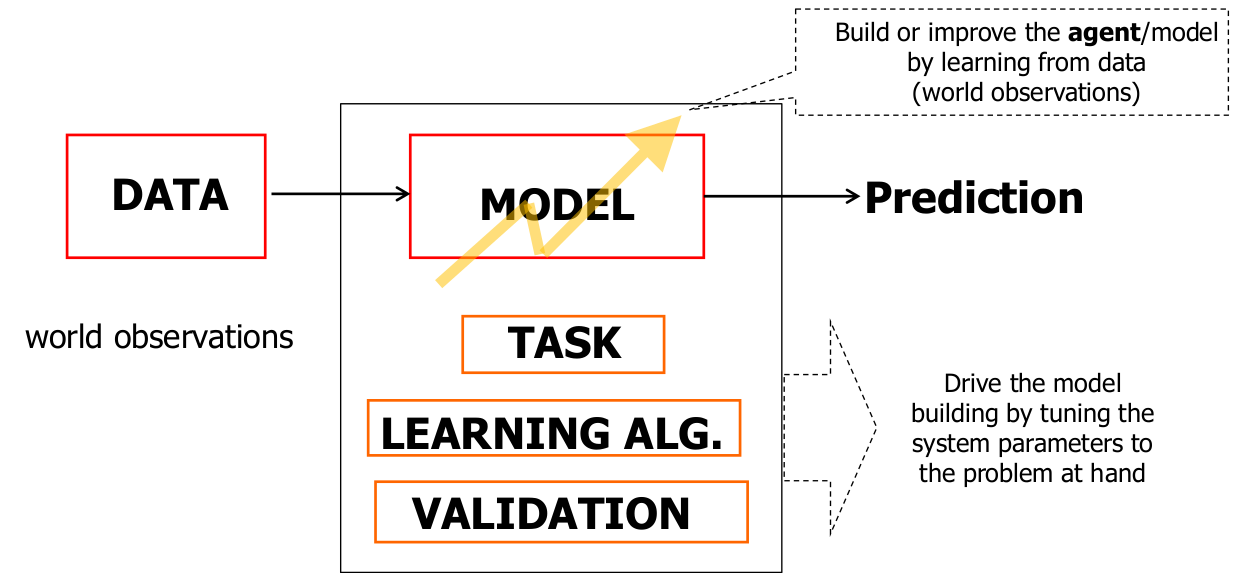
\includegraphics[width=\textwidth]{immagini/machine_learning.png}
	\caption*{Overview of a ML System}
\end{figure}

\subsection{Apprendimento supervisionato}

Dato un esempio di addestramento come $\langle input,\ output \rangle$ = $\langle x,\ d \rangle$ (esempi etichettati)
per una funzione sconosciuta $f$ (nota solo nei punti dati dell'esempio), trova una \textit{buona} approssimazione di $f$ (un'\textit{ipotesi h} che può essere usata per
previsione su dati invisibili $x'$).

\noindent Valore target:\ il valore desiderato \textit{d} o \textit{t} o \textit{y} è dato dall'insegnante secondo $f(x)$; può essere un'etichetta categoriale o numerica.
\begin{itemize}
	\item\textbf{\textit{Classificazione}}:\ $f(x)$ restituisce la classe corretta (presunta) per $x$.\ $f(x)$ è una \textit{funzione a valori discreti} $\in \{1,2,\dots, k\}$ classi.
	\item \textbf{\textit{Regressione}}:\ approssimare una funzione target a valori reali (in $\mathbb{R}$ o $\mathbb{R}^K$)
\end{itemize}

\noindent Entrambi come compito di approssimazione di funzioni.

\subsection{Apprendimento non supervisionato}

Apprendimento senza supervisione:\ nessun insegnante!\
TR (Training Set) = set di dati senza etichetta $\langle x \rangle$.\
Per esempio per trovare \textit{raggruppamenti naturali} in un insieme di dati
\begin{itemize}
	\item Raggruppamento
	\item Riduzione/visualizzazione/pre-elaborazione della dimensionalità
	\item Modellazione della densità dei dati
\end{itemize}

\noindent Clustering:\ partizione dei dati in cluster (sottoinsiemi di dati ``simili'').\ Centroidi:\ centro dei cluster.

\subsection{Modelli e rassegna di concetti utili}

Modello:\ definisce la classe di funzioni che la macchina di apprendimento può implementare (spazio delle ipotesi).\ Obiettivo:\ acquisire/descrivere le relazioni tra i dati (sulla base del compito), per esempio insieme di funzioni $h (x, w)$, dove $w$ è il parametro (astratto).

Esempio di allenamento (superv.)\ della forma $(x, f (x) + rumore)$ $x$ è solitamente un vettore di caratteristiche, (\textit{d} o \textit{t} o) $y = f (x) + rumore$ è chiamato valore target.

\begin{flushleft}
	\textbf{Funzione target}:\ la vera funzione \textit{f}

	\textbf{Ipotesi}:\ una funzione proposta \textit{h} ritenuta simile a \textit{f}.\
	Un'espressione in un determinato linguaggio che descrive le relazioni tra i dati

	\textbf{Spazio ipotesi}:\ lo spazio di tutte le ipotesi (modelli specifici) che possono, in linea di principio, essere emesse dall'algoritmo di apprendimento.
\end{flushleft}

\subsubsection{Esempi di modelli}

Giusto per avere un'anteprima della diversa rappresentazione delle ipotesi:

\begin{itemize}
	\item Modelli lineari (la rappresentazione di H definisce uno spazio continuamente parametrizzato di ipotesi potenziali); ogni assegnazione di \textit{w} è un'ipotesi diversa, ad esempio:
	      \[
		      h_w(x) = w_1 x + w_0
	      \]
	\item Regole simboliche:\ lo spazio delle ipotesi è basato su rappresentazioni discrete; sono possibili regole diverse, ad esempio:
	      \begin{table}[H]
		      \centering
		      \begin{tabular}{l}
			      \textit{if} ($x_1 = 0$) \textit{and} ($x_2 = 1$) \textit{then} $h(x) = 1$ \\
			      \textit{else} $h(x) = 0$                                                  \\
		      \end{tabular}
	      \end{table}
	\item Modelli probabilistici:\ stima $p (x, y)$.
	\item Approcci basati sull'istanza:\ prevedere il valore medio \textit{y} dei vicini più vicini (basato sulla memoria).
\end{itemize}

\subsection{Algoritmi di apprendimento}

Basandosi su dati, task e modello, l'apprendimento come \textit{ricerca} (euristica) a\textit{ttraverso lo spazio delle ipotesi H} dell'\textbf{ipotesi migliore} cioè la migliore approssimazione alla funzione target (sconosciuta).\
\begin{figure}[H]
	\centering
	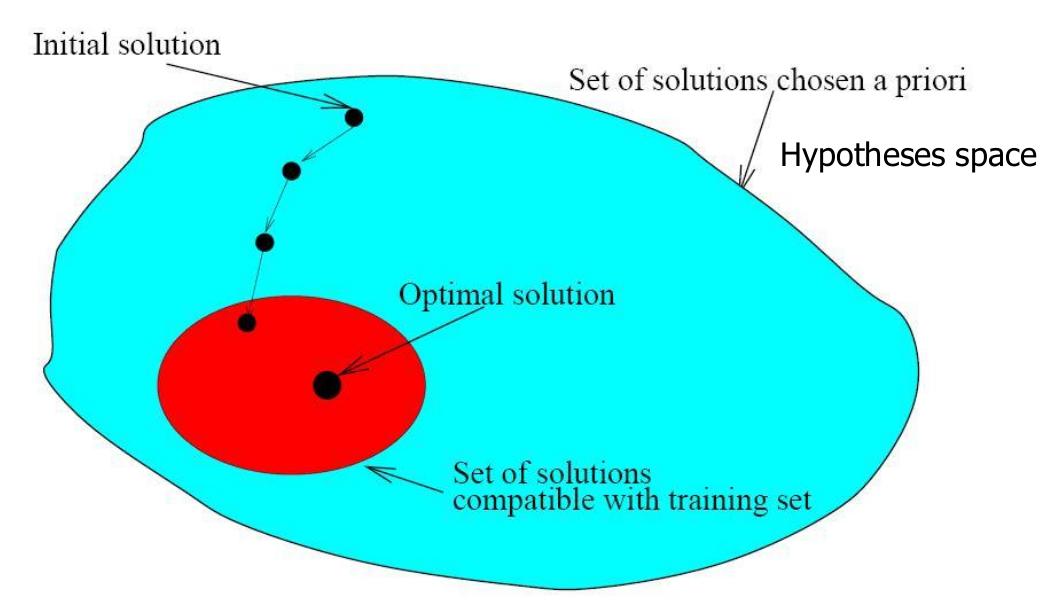
\includegraphics[width=0.5\textwidth]{immagini/ML_search.png}
	\caption*{Ricerca locale}
\end{figure}

\noindent In genere la ricerca della \textit{h} con il minimo ``errore''.\
\textit{H} potrebbe non coincidere con l'insieme di tutte le possibili funzioni e la ricerca non può essere esaustiva:\ bisogna fare delle ipotesi $\rightarrow$ vedremo il ruolo del bias induttivo.

\subsection{Generalizzazione}

\textit{Apprendimento}: ricerca di una \textbf{\textit{buona funzione}} in uno spazio funzionale da dati noti (in genere riducendo al minimo un errore/perdita).\
\textbf{Buona} rispetto all'errore di generalizzazione:\ misura la precisione con cui il modello prevede su nuovi campioni di dati (errore/perdita misurata su nuovi dati, basso errore, alta precisione e viceversa).\
La generalizzazione è il punto cruciale del ML!\
Strumenti ML facili da usare rispetto a un uso corretto del ML.

\noindent\textbf{Fase di apprendimento} (formazione, adattamento):\ costruire il modello da dati conosciuti, di addestramento (e bias).\

\noindent\textbf{Fase predittiva} (test):\ applicare al nuovo esempio (prendiamo l'input x, calcoliamo la risposta dal modello, confrontiamo con il suo obiettivo che il modello non ha mai visto); valutazione dell'ipotesi predittiva, ovvero della \textbf{capacità di generalizzazione}.\

\textbf{Nota}:\ quando parliamo di \textit{prestazioni} in ML ci riferiamo all'\textit{accuratezza predittiva} stimata dall'errore calcolato sul set di test.\
